\chapter{Seguimiento de carriles} \label{cap:seguimiento_de_carriles}
% BREVE DESCRIPCIÓN DEL CONTENIDO DE ESTE CAPÍTULO
Este capítulo se enfoca en hacer un primer reconocimiento del ambiente, se buscan identificar los carriles de la carretera, en especial, el carril donde se encuentra el vehículo autónomo. Al inicio, la sección \ref{sec:introducción_al_seguimiento_de_carriles} realiza una introducción para el proceso de seguimiento de carriles. A continuación, en \ref{sec:el_espacio_de_color_RGB} se define el concepto de espacio de color y algunas de las variantes más utilizadas, en la subsección \ref{sub:ejemplo_para_obtener_la_imagen_de_la_cámara} se muestra una forma de procesar una imagen RGB con la plataforma ROS. Enseguida, las secciones \ref{sec:detección_de_bordes} y \ref{sec:transformada_Hough} tratan de manera teórica los conceptos de detección de bordes de Canny y transformada Hough. Sus correspondientes subsecciones \ref{sub:ejemplo_para_detección_de_bordes_con_el_detector_de_canny} y \ref{sub:ejemplo_para_detección_de_líneas_rectas_con_transformada_Hough} son ejemplos de como implementar estas herramientas matemáticas en código de programación para aplicaciones de vehículos autónomos. Posteriormente, la sección \ref{sec:modelo_cinemático_del_vehículo} es una muestra del modelo cinemático del vehículo, siguiendo este modelo la sección \ref{sec:leyes_de_control} diseña las leyes de control correspondientes para el movimiento lateral y longitudinal del vehículo. Finalmente, se presentan los resultados de estas implementaciones.

Cabe mencionar que todas las implementaciones en código de algoritmos y pseudocódigos propuestos en este capítulo son desarrollados con el lenguaje de programación Python.

\section{Introducción al seguimiento de carriles} \label{sec:introducción_al_seguimiento_de_carriles}

El primer paso para cumplir con la tarea de navegación autónoma es el seguimiento de carriles, en un ambiente vial urbano los carriles son el principal indicador para mantener una ruta. Bajo este escenario, es fundamental contar con un instrumento que permita simular en medida de lo posible la visión humana, el sensor más cercano a este efecto es una cámara, con ella se puede conocer una parte del ambiente donde navegará el vehículo. Tal como se describió en la sección \ref{sec:el_ambiente_de_simulación} del capítulo \ref{cap:simulación_con_webots}, el vehículo autónomo modelado está instrumentado con una cámara digital en la parte superior para tener una imagen RGB frontal del ambiente. La imagen obtenida de la cámara es la principal fuente de información para supervisar el frente de la escena, está información (imagen) es procesada con el fin de identificar el carril donde debe conducir el vehículo autónomo y en base a ello calcular las leyes de control que permitan manipular las funciones operativas (movimiento lateral y longitudinal) del vehículo para mantenerse dentro del carril correspondiente en líneas curvas y rectas de la carretera. Para que el vehículo autónomo sea capaz de navegar bajo estas condiciones es recomendable separar el proceso en tareas más específicas, en concreto dos: Detección de carril y Seguimiento de Carril.

El reconocimiento del ambiente hace referencia a la detección del carril en el que debe mantenerse el vehículo, para realizar esta tarea se llevan a cabo los siguientes pasos:
\begin{enumerate}
    \item Obtener la información (imagen) de la cámara del vehículo.
    \item Determinar características de la imagen que ayuden en la detección del carril.
    \item Identificar las líneas que correspondan a los bordes del carril.
\end{enumerate}

La acción de seguimiento de carril se pretende conseguir mediante:
\begin{enumerate}
    \item Diseño e implementación de un control para velocidad y dirección del vehículo.
    \item Garantizar la seguridad del vehículo en todo momento.
\end{enumerate}

En las siguientes secciones de este capítulo se describen conceptos teórico matemáticos necesarios para el procesamiento digital de imágenes en la búsqueda de detección de carriles en la escena, además se ejemplifican los casos prácticos de cada una de las herramientas empleadas.

\section{El espacio de color RGB} \label{sec:el_espacio_de_color_RGB}

Dentro del procesamiento de imágenes es de suma importancia el uso de color por dos principales razones. En primer lugar, el color es un descriptor muy poderoso para la identificación y extracción de objetos de una escena. Por otra parte, los humanos podemos distinguir entre cientos de tonos de color pero solo un par de docenas en tonos de grises. Así, el procesamiento de imágenes a color se puede dividir en dos categorías: Procesamiento de Pseudo-color y Procesamiento de color completo. Para el procesamiento por Pseudo-color se emplea la asignación de color a una determinada intensidad de escala de grises mientras que en procesamiento de  color completo las imágenes se obtienen con ayuda de algún sensor a todo color(cámara digital, escáner a color) \cite{gonzalez2009digital}.

Un espacio de color es una forma para indicar como está definido un color, el propósito de un espacio de color, modelo de color o sistema de color como también es conocido consiste en facilitar la especificación de colores de una manera estándar. Es decir, es una especificación de un sistema de coordenadas y un sub-espacio dentro del sistema, de tal modo que cada color está representado por un solo punto contenido dentro del sub-espacio. En la práctica de procesamiento de imágenes los modelos de color más utilizados son el modelo RGB (Red, Green, Blue) para monitores de color, cámaras de vídeo; los modelos CMY (Cyan, Magenta, Yellow) y CMYK (Cyan, Magenta, Yellow, Black) son muy usados dentro de la industria de impresión de color. El modelos HSI (Hue, Saturation, Intensity) es el modelo que más se asemeja a la forma en que los humanos interpretamos el color, este modelo tiene la ventaja de poder desacoplar el color y el gris(escala de grises de una imagen) y por lo tanto es bastante común en el uso de técnicas de escala de grises\cite{gonzalez2009digital}.

El modelo de color RGB se basa en un sistema cartesiano de 3 coordenadas y el sub-espacio de interés es un cubo unitario. Es decir, se indica que todos los valores R, G y B se encuentran en un rango de [0, 1]. Dentro del espacio RGB, cada color aparece en su componente espectral primaria(R = 645.16nm, G = 526.32nm , B = 444.44nm)\cite{levinson2011towards}. El color negro se encuentra en el origen del cubo mientras que el blanco está situado en el vértice más lejano, los valores primarios (RGB) se sitúan en tres esquinas del cubo y los colores secundarios aparecen en las tres esquinas restantes. Los diferentes colores sobre o dentro del cubo están definidos por vectores que comienzan desde el origen. Además, la escala de grises (puntos donde los valores RGB son iguales) se extiende de negro a blanco a través de la línea que une estos dos vértices. La figura \ref{fig:rgb_cube} muestra la representación del espacio de color RGB.
\begin{figure}[h]
    \centering
    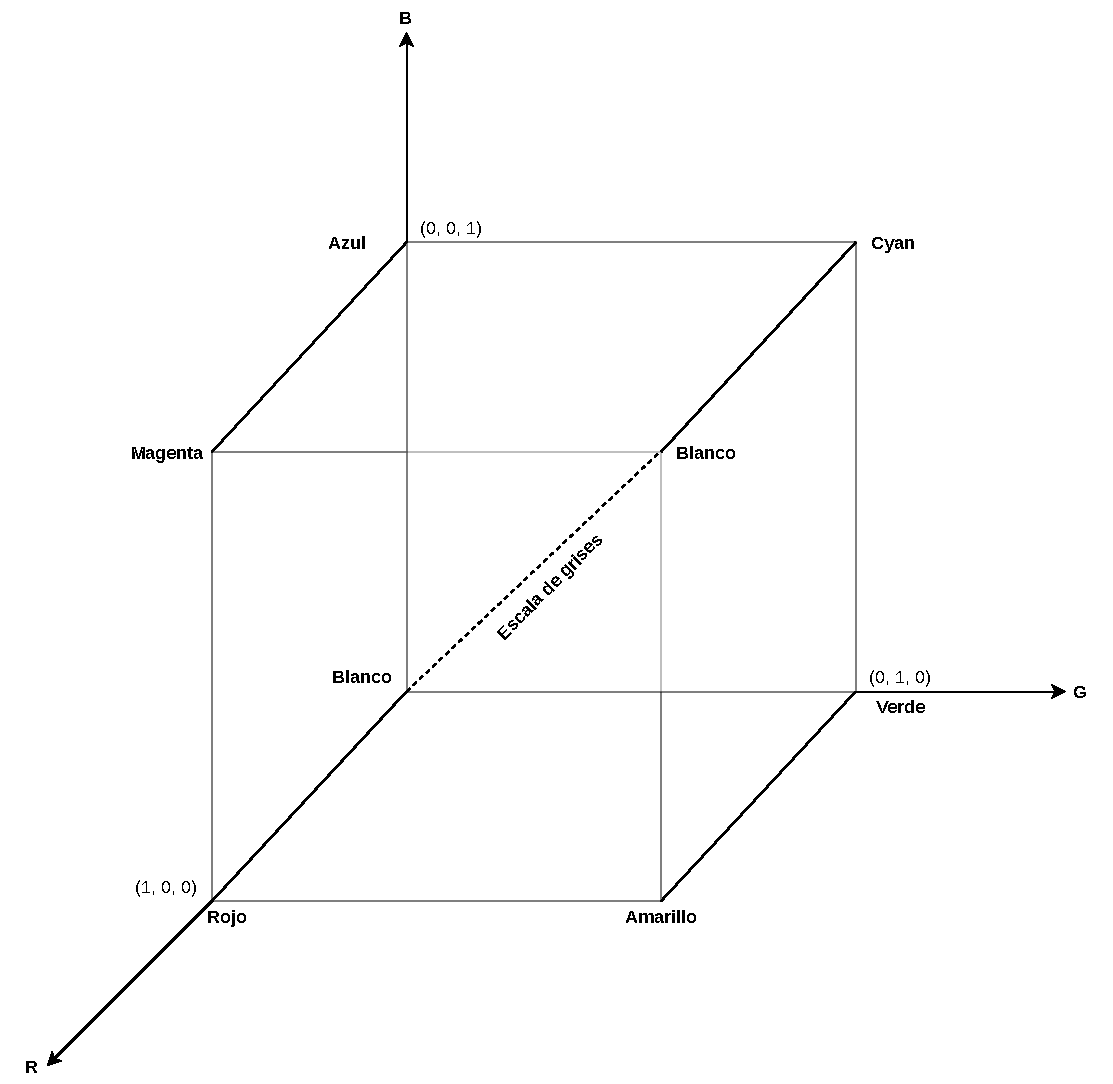
\includegraphics[width=0.75\textwidth]{Figures/Figures_Cap04/rgb_cube.pdf}
    \caption{Espacio RGB en coordenadas cartesianas.}
    \label{fig:rgb_cube}
\end{figure}

\subsection{Ejemplo para obtener la imagen de la cámara} \label{sub:ejemplo_para_obtener_la_imagen_de_la_cámara}

La cámara del vehículo provee una imagen en formato RGBA de 8-bits con dimensiones de ``640x480'' píxeles. A fin de obtener la imagen son necesarias las funciones especificas del nodo ``Camera'' del simulador Webots, además se hace uso de la plataforma ROS para el manejo de tópicos entre diferentes nodos, en específico se utiliza un mensaje del tipo \textit{Image} de ROS con la intención de publicar un tópico que contenga la información de la cámara. 

Para comenzar el procesamiento de la imagen se realiza una conversión de el mensaje \textit{Image} de ROS a una imagen tipo CV2 de OpenCV. Esto porque el mensaje \textit{Image} de ROS contiene la información de imagen en forma de lista donde el tamaño corresponde a el número de píxeles de la imagen (ancho por alto), en este caso el tamaño de la lista es de 640x480 = 307200. Cada uno de los elementos de la lista representa un píxel de la imagen en formato ARGB de 32 bits.

OpenCV es una biblioteca de código abierto para manipulación y procesamiento de imágenes, en adición con la alta compatibilidad entre la plataforma ROS y OpenCV son las principales razones para usar OpenCV dentro de este proyecto pues las funciones que ofrece son suficientes para cada uno de los pasos en el diseño de un algoritmo de detección carriles. Dentro de la plataforma ROS se encuentra un paquete llamado ``cv\_bridge'' el cual permite la conversión bilateral entre mensajes del tipo \textit{Image} de ROS e imágenes en formato OpenCV. La imagen \ref{fig:cv_bridge} ejemplifica la conversión entre estos dos tipos de mensajes.
% \footnote{\url{http://wiki.ros.org/cv_bridge/Tutorials}}
\begin{figure}
    \centering
    \begin{subfigure}[b]{0.4\textwidth}
         \centering
        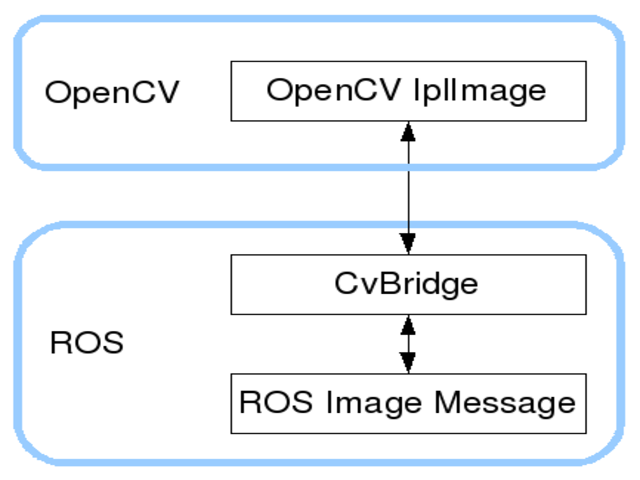
\includegraphics[width=\textwidth]{Figures/Figures_Cap04/cvbridge.png}
        \caption{Mensaje \textit{Image} de ROS a imagen de OpenCV.}
        \label{fig:cv_bridge}
    \end{subfigure}
    \hfill
    \begin{subfigure}[b]{0.4\textwidth}
        \centering
        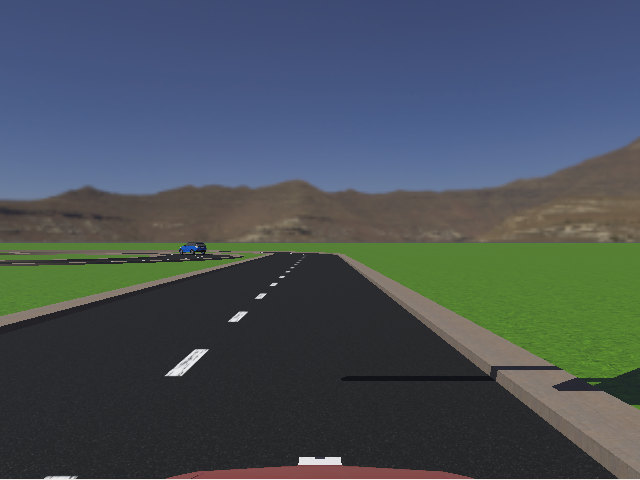
\includegraphics[width=\textwidth]{Figures/Figures_Cap04/lanes.png}
        \caption{Imagen de la cámara en formato de OpenCV.}
        \label{fig:lanes_cv}
    \end{subfigure}
    \caption{Resultado de transformar un mensaje \textit{Image} de ROS a una imagen de OpenCV.}
    \textit{Nota}. (a) Tomada de \textit{Stechschulte}, 2020 \cite{cv_bridge}.
    \label{fig:ros_cv}
\end{figure}

Referente a la implementación de código, la principal fuente información es proporcionada en la documentación oficial de OpenCV, disponible en \footnote{\url{https://opencv.org/}}. A continuación se muestra el código necesario para el tratado de un mensaje \textit{Image} de ROS y la conversión a imagen de OpenCV. En \ref{fig:lanes_cv} se ilustra el resultado de la imagen obtenida.

\begin{lstlisting}[language=Python]
from cv_bridge import CvBridge

bridge = CvBridge()
cv2_img = bridge.imgmsg_to_cv2(msg, 'bgr8')
\end{lstlisting}

\section{Detección de bordes} \label{sec:detección_de_bordes}

La detección de bordes es una herramienta en el procesamiento de imágenes diseñada para detectar píxeles de borde. Los píxeles de borde son píxeles donde la intensidad de una imagen cambia abruptamente y los bordes son conjuntos de píxeles entre bordes conectados. Es decir, la detección de bordes se utiliza para segmentar imágenes en función de cambios bruscos de intensidad. 

Dentro de este contexto existen diferentes formas de modelar un borde, una muy utilizada clasificación es usar como criterio la intensidad. Este escenario contempla: \textit{Step Edge} o borde de paso, como aquél que se presenta cuando existe una transición entre dos niveles de intensidad en distancia de un píxel. En la práctica es muy común encontrar imágenes distorsionadas por ruido o por algún filtro añadido previamente, de manera coloquial se entiende que la imagen se ve borrosa. En tales situaciones se pueden modelar bordes mediante una rampa de intensidad \textit{Ramp Edge}, donde la pendiente de la rampa es inversamente proporcional al grado de desenfoque, ya que no se cuenta con un solo punto de borde, cada punto dentro de la rampa es un punto borde aceptable, de esta manera un segmento de borde es un conjunto de puntos situados en la rampa. Como tercer tipo de borde está \textit{Roof Edge} o borde de techo, los bordes de techo son modelos de líneas dentro de una región, donde el ancho del borde es determinado por medio del grosor y nitidez de la línea, es normal encontrar bordes de techo en digitalización de dibujos e imágenes satélites\cite{gonzalez2009digital}. La figura \ref{fig:edges_types} ejemplifica los tres tipos de bordes descritos.
% \footnote{\url{https://www.ics.uci.edu}}
\begin{figure}[h]
    \centering
    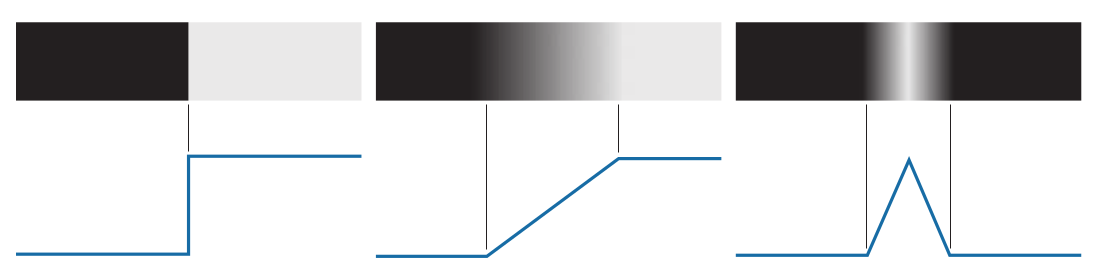
\includegraphics[width=0.75\textwidth]{Figures/Figures_Cap04/edge_type.png}
    \caption{Tipos de Bordes.}
    \textit{Nota}. Tomada de \textit{Gonzalez}, 2009 \cite{gonzalez2009digital}.
    \label{fig:edges_types}
\end{figure}

Los bordes mencionados anteriormente son los más comunes y utilizados por algoritmos de detección de bordes, debido a que son comportamientos muy frecuentes en imágenes. En general, un algoritmo de detección de bordes consta de tres pasos esenciales:
\begin{enumerate}
    \item Suavizar la imagen para reducir ruido.
    \item Detectar puntos borde (Puntos potenciales para ser candidatos a puntos de borde).
    \item Localizar bordes (Selección de puntos candidatos que pertenecen a un borde).
\end{enumerate}

\subsection{Detector de bordes de Canny} \label{sub:detector_de_bordes_de_canny}

Desarrollado en 1986 por John F. Canny, es un algoritmo para detección de bordes con mayor complejidad que los algoritmos tradicionales. Sin embargo, el rendimiento de este también resulta ser superior. El enfoque de este algoritmo se basa en tres principales objetivos:
\begin{enumerate}
    \item Tasa de error baja. Se deben localizar todos los bordes y no deben existir respuestas ilegítimas.
    \item Los puntos borde deben ser bien ubicados. Los bordes detectados deben estar lo más cercano posible a los bordes verdaderos. Es decir, debe existir distancia mínima entre ellos.
    \item Respuesta única de punto de borde. El detector debe devolver solo un punto borde por cada punto de borde verdadero. 
\end{enumerate}

El funcionamiento para detección de bordes mediante el algoritmo de Canny se fundamenta en el uso del vector gradiente debido a que este vector cuenta con la conocida propiedad de apuntar en la dirección de máxima tasa de cambio \cite{gonzalez2009digital}. El vector gradiente de una imagen se define en la ecuación (\ref{eqn:img_gradient}):
\begin{equation}
    \nabla f(x, y) \equiv grad[f(x, y)] \equiv \begin{bmatrix} 
        g_x(x, y) \\
        \\
        g_y(x, y) 
    \end{bmatrix}
    = 
    \begin{bmatrix} 
        \frac{\partial f(x, y)}{\partial x}\\
        \\
        \frac{\partial f(x, y)}{\partial y}
    \end{bmatrix}
    \label{eqn:img_gradient}
\end{equation}

Esta herramienta permite determinar la magnitud y dirección de un borde, donde la magnitud $M(x, y)$  es el valor de la tasa de cambio en la dirección del gradiente y está compuesta por su norma vectorial euclidiana.
\begin{equation}
    M(x, y) = \nabla \|f(x, y)\| = \sqrt{g_x^2(x, y) + g_y^2(x, y)}
\end{equation}

La dirección del vector gradiente en un punto $(x, y)$ está dada por:
\begin{equation}
    \alpha (x, y) = \tan^{-1} \begin{bmatrix}
        \frac{g_y(x, y)}{g_x(x, y)}
    \end{bmatrix}
\end{equation}

El algoritmo para detección de bordes de Canny consta de los siguientes pasos.
\begin{enumerate}
    \item Aplicar filtro gaussiano a la imagen de entrada para disminuir ruido.
    \item Calcular magnitud y ángulo del vector gradiente.
    \item Suprimir puntos no máximos.
    \item Detectar y vincular bordes mediante aplicación de doble umbralización.
\end{enumerate}

\subsection{Ejemplo para detección de bordes con el detector de Canny} \label{sub:ejemplo_para_detección_de_bordes_con_el_detector_de_canny}

%Se puede afirmar que los bordes son una poderosa característica para obtener información concreta de una escena. En la detección de carriles como primer paso se pretenden calcular los bordes contenidos en toda la imagen con el fin de contar con elementos suficientes que describan cada uno de los objetos presentes. 
El algoritmo de bordes de Canny es la herramienta seleccionada para lograr el proceso de extraer los bordes que representan los carriles de la carretera, en específico las líneas que conforman los bordes del carril donde se encuentra el auto de pruebas. OpenCV provee una función para utilizar el algoritmo de Canny, en breve se presenta la sección de código donde se hace uso de la función ``Canny()'' de OpenCV.

\begin{lstlisting}[language=Python]
import cv2

def canny(image):

    gray = cv2.cvtColor(image, cv2.COLOR_RGB2GRAY)  
    blur = cv2.GaussianBlur(gray, (5, 5), 0)        
    canny = cv2.Canny(blur, 50, 150)                
    return canny
\end{lstlisting}

El código anterior expone la forma de usar la función ``Canny()'' de OpenCV para detección de bordes. En la primer sentencia (línea 5) se realiza una conversión entre espacios de color, en específico de una imagen RGB a una imagen en escala de grises, el segundo paso (línea 6) tiene aplica un filtro Gaussiano a la imagen en escala de grises para reducir ruido. Finalmente en la línea 7 se aplica en concreto la función 'cv2.Canny()' para obtener una imagen en blanco y negro que contiene los bordes detectados por ``Canny()''.

La imagen \ref{fig:lanes_comparsion}, ofrece una comparación entre la imagen original \ref{fig:lanes} obtenida de la cámara y la imagen de bordes alcanzada por el algoritmo de Canny \ref{fig:edges_lanes}. El resultado de está operación es muy importante para el siguiente paso en la detección los carriles.
\begin{figure}[h]
    \centering
    \begin{subfigure}[b]{0.4\textwidth}
         \centering
         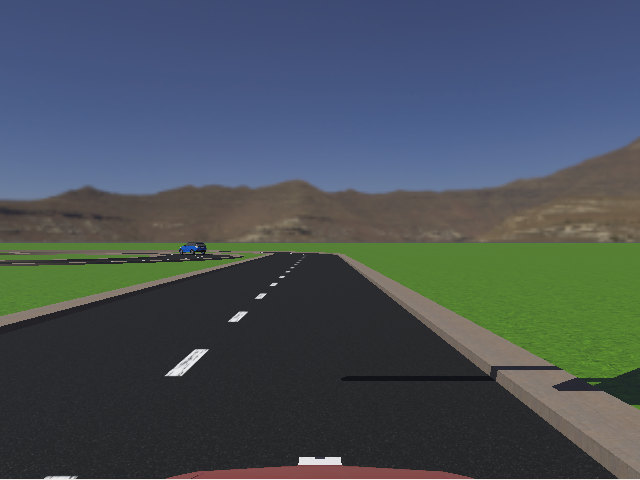
\includegraphics[width=\textwidth]{Figures/Figures_Cap04/lanes.png}
         \caption{Imagen original.}
         \label{fig:lanes}
    \end{subfigure}
    \hfill
    \begin{subfigure}[b]{0.4\textwidth}
         \centering
         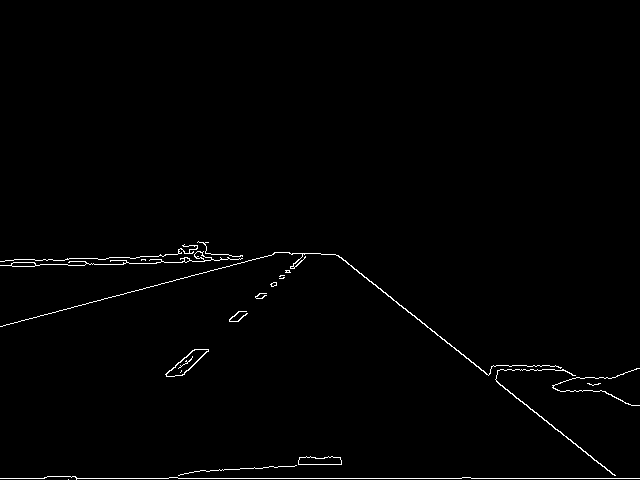
\includegraphics[width=\textwidth]{Figures/Figures_Cap04/edge_lanes.png}
         \caption{Imagen de Bordes.}
         \label{fig:edges_lanes}
     \end{subfigure}
     
    \caption{Comparación en entre la imagen original y la imagen de bordes.}
    \label{fig:lanes_comparsion}
\end{figure}

\section{Transformada Hough} \label{sec:transformada_Hough}

Buscar formas dentro de una imagen digital es una tarea común en el procesamiento de imágenes, en muchas de las ocasiones se buscan ajustar un conjunto de puntos en una determinada estructura, ya sean líneas rectas, círculos o alguna otra geometría. La transformada de Hough es una técnica propuesta por Paul Hough en 1962 y ampliamente utilizada dentro del campo de visión computacional para detección de líneas rectas y curvas en imágenes a color y en escala de grises.

El algoritmo busca identificar formas básicas en una imagen haciendo uso de los parámetros que describen la geometría deseada. Dentro de este concepto la transformada de Hough funciona a través de un sistema de votación, es decir, se identifica una forma específica si se obtiene un número suficiente de votos. Mediante esta técnica es posible encontrar cualquier figura que pueda ser expresada matemáticamente, el caso más sencillo es la detección de líneas rectas \cite{forsyth2011computer}.

\subsection{Detección de líneas rectas mediante transformada Hough} \label{sub:detección_de_líneas_rectas_mediante_transformada_Hough}

Dentro del espacio de imagen una línea puede ser expresada en un sistema cartesiano mediante los parámetros $(m, b)$ con la ecuación:
\begin{equation}
    y = mx + b
\end{equation}
mientras que en un sistema polar con los parámetros $(\rho, \theta)$ como:
\begin{equation}
    \rho = x \cos{\theta} + y \sin{\theta}
    \label{eqn:polar_line} 
\end{equation}

El principio fundamental del algoritmo de Hough para detección de líneas rectas consiste en trazar $n$ cantidad de líneas rectas para cada punto de la imagen y mediante el sistema de votación determinar que puntos forman una línea. Para la transformada de Hough resulta más sencillo trabajar en un sistema polar con los parámetros $(\rho, \theta)$, debido a que para cualquier punto de la imagen existen una infinidad de líneas que pasan a través de él, en el caso de líneas verticales los parámetros $(m, b)$ están indefinidos, en un sistema polar no existe este problema pues para líneas verticales se tiene $\theta = 90^\circ$ y para líneas horizontales $\theta = 0^\circ$. De esta manera se evita cualquier tipo de discontinuidad. Además, en la forma polar si la línea corresponde a un borde, el ángulo $\theta$ es la dirección del gradiente \cite{gonzalez2009digital}.

Como se mencionó anteriormente en cada punto de la imagen se trazan $n$ líneas, teniendo en cuenta esto es evidente que al menos una de las $n$ líneas atraviesa dos o más puntos de la imagen, es decir, los puntos sobre la recta tienen la propiedad de ser colineales, este es el sistema de votación que utiliza el algoritmo de Hough, pues entre más puntos estén contenidos dentro de una recta más votos tendrá, como consecuencia la recta con el mayor número de votos será considerada como una línea recta identificada dentro de la imagen.

Tomado como ejemplo la imagen \ref{fig:cartesian_space} se tienen dos puntos $(x_i, y_i)$ y $(x_j, y_j)$ en el espacio de imagen contenidos en el plano $xy$, la recta azul $L$ representa una recta en forma polar con parámetros $(\rho, \theta)$ que pasa a través de los puntos $(x_i, y_i)$ y $(x_j, y_j)$. Esta línea $L$ en el espacio cartesiano corresponde a un punto $P_h$ en el espacio de Hough con coordenadas $(\rho', \theta')$ en \ref{fig:hough_space}. Un punto $P(x_i, y_i)$ en el espacio cartesiano corresponde a una curva $C_i$ en el espacio de Hough, donde $C_i$ es  representada por los parámetros $(\rho_i, \theta_i)$ de todas las rectas $L_i$ que pasan por el punto $P(x_i, y_i)$ en el espacio cartesiano calculados mediante la ecuación (\ref{eqn:polar_line}), la imagen \ref{fig:hough_space} muestra la familia de curvas $C$ que pasan a través del punto $P_h$ en el espacio de Hough.

Finalmente el método de votación del algoritmo de Hough consiste en encontrar las curvas $C_i$ dentro del espacio de Hough que pasan a través del punto $P(x_i, y_i)$ del espacio cartesiano. Los puntos $P_h$, es decir la intersección $(\rho ', \theta')$ en el espacio de Hough por donde pasen más curvas $C_i$ serán las rectas resultantes en el espacio cartesiano.
\begin{figure}
    \centering
    \begin{subfigure}[b]{0.4\textwidth}
         \centering
         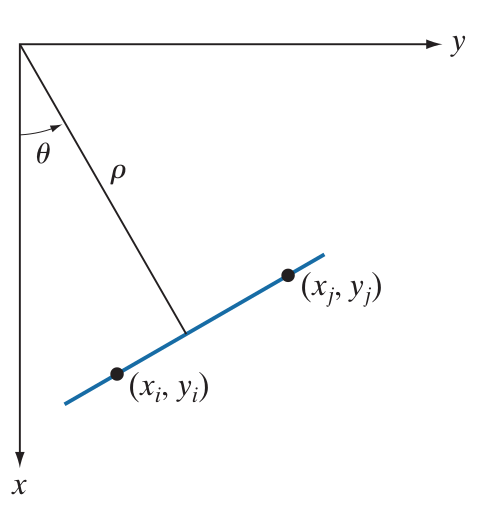
\includegraphics[width=\textwidth]{Figures/Figures_Cap04/cartesian_space.png}
         \caption{Parametrización de una recta en el plano $xy$.}
         \label{fig:cartesian_space}
    \end{subfigure}
    \hfill
    \begin{subfigure}[b]{0.42\textwidth}
         \centering
         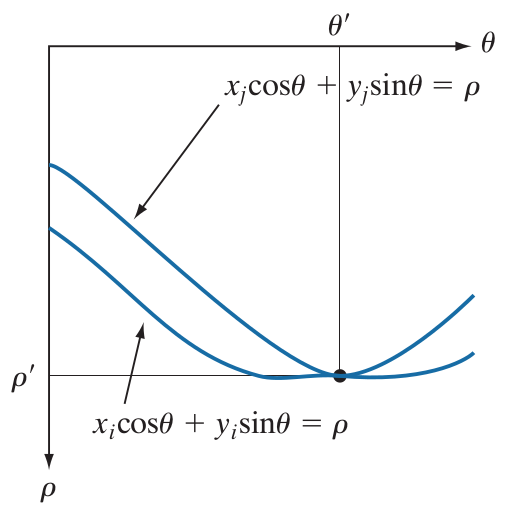
\includegraphics[width=\textwidth]{Figures/Figures_Cap04/hough_space.png}
         \caption{Familia de Curvas en el espacio de Hough.}
         \label{fig:hough_space}
     \end{subfigure}
     
    \caption{Interpretación geométrica de los espacios cartesiano y de Hough.}
    \textit{Nota}. Tomadas de \textit{Gonzalez}, 2009 \cite{gonzalez2009digital}.
    \label{fig:cartesian_hough_space}
\end{figure}

\subsection{Ejemplo para detección de líneas rectas con transformada Hough} \label{sub:ejemplo_para_detección_de_líneas_rectas_con_transformada_Hough}

Para continuar con el proceso de detección de carril es necesario identificar las líneas que los conforman, ver \ref{fig:lanes}. La manera más sencilla de encontrar un carril dentro de una imagen es delimitar el espacio donde se encuentra. Un carril está contenido por dos líneas rectas paralelas que pueden ser continuas, discontinuas e incluso líneas rectas dobles. El problema que se presenta en este caso es la detección de líneas rectas y el enfoque de la transformada de Hough para líneas rectas es justo la herramienta que permite resolver este problema. 

Los párrafos siguientes describen una forma en que se puede usar la transformada de Hough para detección de líneas rectas e identificar las líneas que forman un carril.

Es importante mencionar que la transformada de Hough para detección de líneas rectas produce un mejor resultado con una imagen que presente solo la información de los bordes y en una escala de grises o bien en blanco y negro, este requisito justifica el hecho de haber detectado los bordes de la imagen de la cámara del vehículo de pruebas con el algoritmo de Canny, pues con está imagen se obtendrán las líneas que forman el carril donde se encuentra el vehículo. Sin embargo, no todos los bordes de la imagen son necesarios, por ello es necesario delimitar solo el área de interés donde se encuentra el carril, una vez determinada el área de interés es más fácil y eficiente obtener las líneas pertenecientes al carril.

El proceso de detección de carril mediante líneas rectas requiere definir el área donde está situado el carril de interés, este procedimiento se describe a continuación:
\begin{enumerate}
    \item Obtener una imagen con los bordes de la imagen original, ver \ref{fig:edge_lines}.
    
    \item Delimitar el perímetro donde se encuentra el carril a través de una geometría que pueda ser descrita mediante líneas rectas. Un triángulo es la geometría que mejor se adecua en este caso particular ver, \ref{fig:triangle_interest}.
    
    \item Descartar los bordes que se encuentren fuera de la región de interés para solo contar con los bordes que corresponden a la geometría del carril, ver \ref{fig:lanes_interest}.
\end{enumerate}

\begin{figure}[h]
    \centering
    \begin{subfigure}[b]{0.3\textwidth}
         \centering
         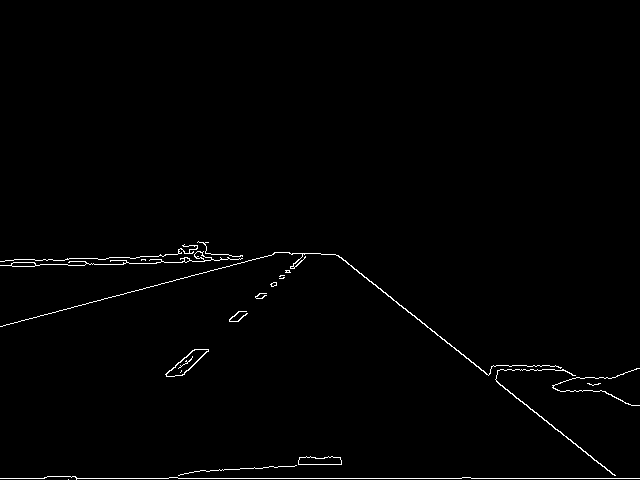
\includegraphics[width=\textwidth]{Figures/Figures_Cap04/edge_lanes.png}
         \caption{Imagen de bordes.}
         \label{fig:edge_lines}
    \end{subfigure}
    \hfill
    \begin{subfigure}[b]{0.3\textwidth}
         \centering
         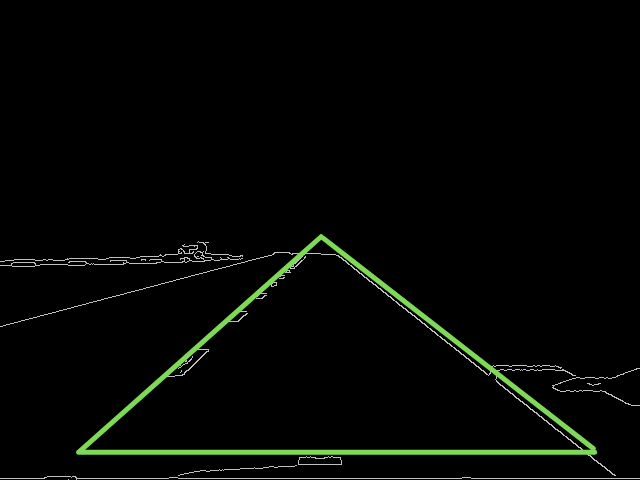
\includegraphics[width=\textwidth]{Figures/Figures_Cap04/triangle_of_interest.png}
         \caption{Triángulo de interés.}
         \label{fig:triangle_interest}
     \end{subfigure}
     \hfill
     \begin{subfigure}[b]{0.3\textwidth}
         \centering
         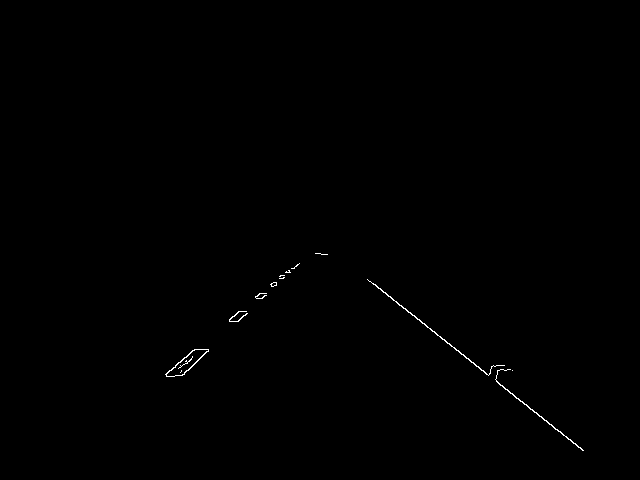
\includegraphics[width=\textwidth]{Figures/Figures_Cap04/lanes_cropped.png}
         \caption{Bordes de interés.}
         \label{fig:lanes_interest}
     \end{subfigure}
     
    \caption{Proceso para delimitar la región de interés de el carril.}
    \label{fig:interest_region}
\end{figure}

\newpage
Previamente se realizó la detección de bordes en la imagen. Ahora es turno de delimitar la zona del carril, la implementación en código para definir el área de interés es la siguiente:

\hfill
\begin{lstlisting}[language=Python]
import cv2
import numpy as np

def region_of_interest(image):
    triangle = np.array( [ (0, 450), (640, 450), (320, 250) ])
    mask = np.zeros_like(image)
    cv2.fillPoly(mask, triangle, 255)
    cropped_img = cv2.bitwise_and(image, mask)
    
    return cropped_img

canny_img = canny(lane_img)                                                 
cropped_img = region_of_interest(canny_img)         
\end{lstlisting}
\hfill

Donde la línea 12 contiene la imagen de bordes obtenidos de la imagen original. A partir de la línea 4 se define la función ``region\_of\_interest()'' para calcular la región de interés, esta función recibe como parámetro la imagen de bordes. En la línea 5 se forma el perímetro del triángulo que contiene los bordes necesarios para identificar el carril, por último la línea 8 secciona la imagen de bordes y solo permanecen los bordes que forman el carril de interés. En \ref{fig:lanes_interest} se ilustra el resultado de la ejecución de este desarrollo.

La tarea más importante en la detección de las líneas que forman el carril es el uso de la transformada Hough para líneas rectas, en breve se enuncian los pasos para obtener las líneas resultantes de el carril.

\begin{enumerate}
    \item Aplicar transformada de Hough a la imagen que contiene los bordes de la región de interés.
    \item Identificar las líneas resultantes con el propósito de saber a que borde del carril pertenecen (izquierdo o derecho).
    \begin{itemize}
        \item Para obtener el conjunto de líneas pertenecientes a cada borde se utiliza la pendiente de las rectas detectadas con Hough como diferenciador. En el caso rectas pertenecientes al borde izquierdo del carril $m > 0$, es decir, pendiente positiva y para el borde derecho se tienen rectas con $m < 0$, pendiente negativa. Líneas horizontales son despreciadas.
    \end{itemize}
    \item Obtener un promedio para cada conjunto de líneas debido a que el carril de una carretera cuenta con solo dos líneas rectas (izquierda y derecha), por esta razón es necesario obtener una sola línea del conjunto de rectas pertenecientes a cada grupo que se ajuste bien en cada borde del carril.
    \item Ilustrar el resultado final de las dos líneas rectas con coordenadas cartesianas para comprobar que la detección de carril es correcta.
\end{enumerate}

La línea 1 en la siguiente porción de código es la forma de usar la función que provee OpenCV para la transformada de Hough, donde su primer parámetro es la imagen de bordes pertenecientes a la región del carril que se obtuvo previamente, los parámetros restantes son constantes que requiere la función, estos valores son recomendados en la documentación de OpenCV. Como efecto de esta operación se extraen las líneas rectas detectadas, estas líneas se ilustran en la figura \ref{fig:hough_lines}.

\hfill
\begin{lstlisting}[language=Python]
lines = cv2.HoughLinesP(
            cropped_img,
            2,
            np.pi/180,
            80,
            minLineLength=40,
            maxLineGap=50
        )
\end{lstlisting}
\hfill

Como lo indican los pasos descritos en está sección se deben de filtrar las líneas detectadas en dos grupos (izquierdas y derechas) para poder calcular un promedio por grupo y generar una sola línea en cada borde del carril. La función que realiza este proceso es la siguiente:

\hfill
\begin{lstlisting}[language=Python]
def avg_slope_intercept(image, lines):
    if angle < -0.3 or angle > 0.3:
        if slope < 0:
            right_fit.append((slope, intercept))    
        else:
            left_fit.append((slope, intercept)) 
    
    left_line_avg = np.average(left_fit, axis=0)    
    right_line_avg = np.average(right_fit, axis=0) 
\end{lstlisting}
\hfill

Donde la distribución de líneas detectadas en cada grupo se inicia en la línea 2, en primer lugar se desprecian aquellas líneas con ángulo de inclinación $\theta$ en rango de [-0.3, 0.3] radianes porque estás líneas representan aquellas que son horizontales o están muy cerca de ser horizontales y pueden provocar imprecisiones en el resultado final. A partir de la línea 3 se inicia la condición para dividir en grupos de rectas izquierdas o derechas con la pendiente como diferenciador, $m < 0$ para líneas rectas del borde derecho y $m > 0$ para líneas rectas del borde izquierdo. Finalmente las líneas 8 y 9 contienen el resultado de calcular el promedio de las líneas del borde derecho e izquierdo respectivamente y como consecuencia tener una sola línea por borde tal como se muestra en \ref{fig:avg_lines}. Para ejemplificar el resultado final de la detección de carriles se genera la imagen \ref{fig:combo_img}, donde se muestra la imagen original, las líneas del carril detectadas son colocadas en color azul, esta imagen permite demostrar que la detección del carril funciona correctamente, pues las líneas rectas detectadas se encuentran sobrepuestas en el carril real.
\begin{figure}[h]
    \centering
    \begin{subfigure}[b]{0.3\textwidth}
         \centering
         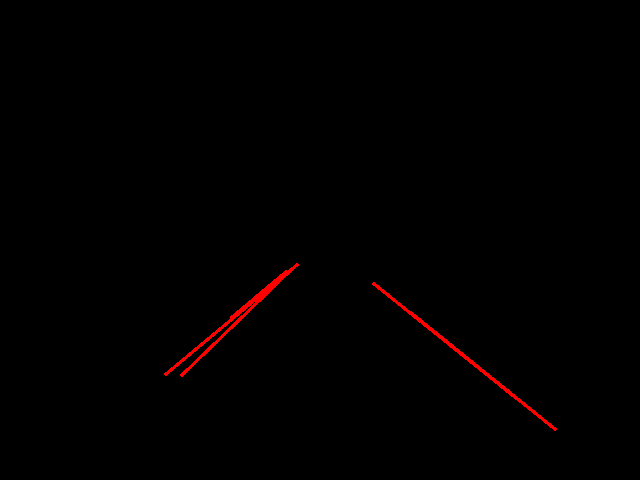
\includegraphics[width=\textwidth]{Figures/Figures_Cap04/hough_lines.png}
         \caption{Líneas detectadas.}
         \label{fig:hough_lines}
    \end{subfigure}
    \hfill
    \begin{subfigure}[b]{0.3\textwidth}
         \centering
         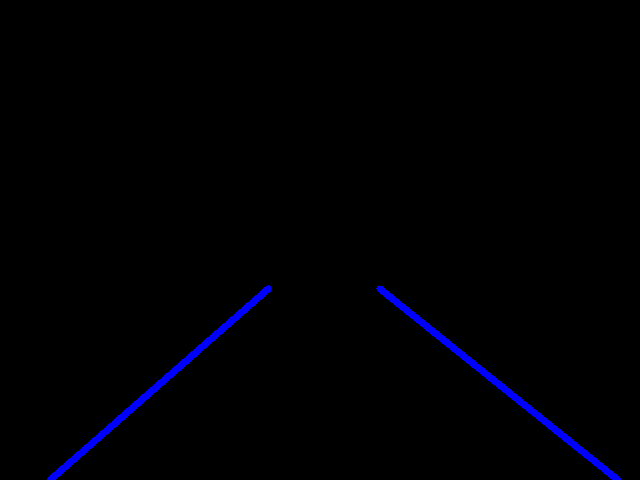
\includegraphics[width=\textwidth]{Figures/Figures_Cap04/avg_hough_lines.png}
         \caption{Líneas promedio.}
         \label{fig:avg_lines}
     \end{subfigure}
     \hfill
     \begin{subfigure}[b]{0.3\textwidth}
         \centering
         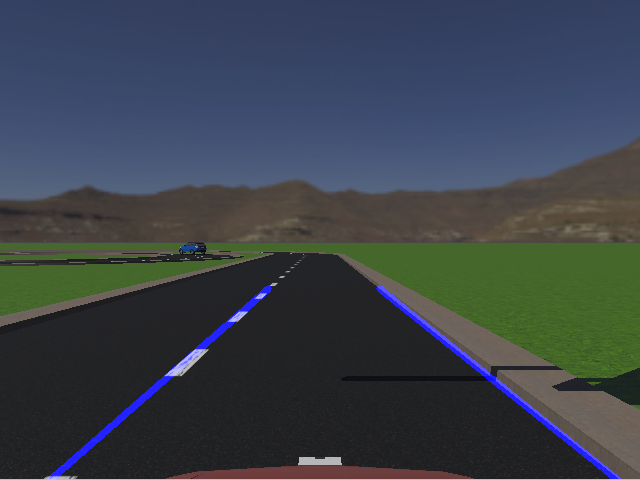
\includegraphics[width=\textwidth]{Figures/Figures_Cap04/combo_img.png}
         \caption{Carril detectado.}
         \label{fig:combo_img}
     \end{subfigure}
     
    \caption{Líneas del carril detectadas por medio de Transformada Hough.}
    \label{fig:lane_detect}
\end{figure}

El resultado del proceso de detección de carril finaliza con la obtención de las líneas que conforman los bordes del carril en coordenadas cartesianas. Estas líneas servirán como modelo en el cálculo de las leyes de control para la tarea de seguimiento de carril donde se involucra velocidad y ángulo de dirección.

\section{Modelo cinemático del vehículo} \label{sec:modelo_cinemático_del_vehículo}

El modelo cinemático es una descripción del movimiento realizado por el Robot en función de su geometría. La cinemática del Robot puede utilizarse como modelo matemático de partida en el diseño de un controlador, para simular el comportamiento cinemático, o para establecer ecuaciones en cálculos de odometría \cite{martinez2003modelado}. 

Para el caso del modelo cinemático del vehículo autónomo se considera el llamado modelo de vía única o \textit{Single-Track-Model} en inglés. En el modelo de única vía, el vehículo cuenta con dos ruedas que están unidas a través de un eslabón que está comprometido a moverse en un plano. Se parte del supuesto que las ruedas pueden girar libremente sobre sus ejes de rotación y que las ruedas no patinan sobre el punto de contacto con el suelo. Además, para modelar la dirección (\textit{steering}) la rueda delantera cuenta con un grado adicional de libertad que le permite girar sobre un eje normal al plano de movimiento. Con estas dos características se refleja la experiencia que tienen los conductores cuando el vehículo no realiza movimiento lateral sin previamente haber avanzado \cite{paden2016survey}. 

Considerando la figura \ref{fig:single_track_model}, donde $p_r$ y $p_f$ son los puntos de contacto con el suelo para los neumáticos trasero y delantero respectivamente, $\theta$ es el ángulo que describe la dirección hacia donde mira el vehículo y $\delta$ es el ángulo de dirección para la rueda delantera. Todo esto en un sistema de coordenadas inercial con vectores base $(\hat{e}_{x}, \hat{e}_{y})$.
% La limitación de maniobras en este modelo se denomina restricción no holonómica y es una restricción diferencial sobre el movimiento del vehículo.
Para satisfacer el supuesto de no deslizamiento, el movimiento de los puntos $p_r$ y $p_f$ debe de ser colineal respecto a la orientación de la rueda. Esta restricción para la llanta trasera se expresa como:
\begin{equation}
    (\dot{p}_r \cdot \hat{e}_y)\cos{(\theta)} - (\dot{p}_r \cdot \hat{e}_x)\sin{(\theta)} = 0
\end{equation}
y para la llanta delantera:
\begin{equation}
    (\dot{p}_f \cdot \hat{e}_y)\cos{(\theta + \delta)} - (\dot{p}_f \cdot \hat{e}_x)\sin{(\theta + \delta)} = 0
\end{equation}

\begin{figure}[h]
    \centering
    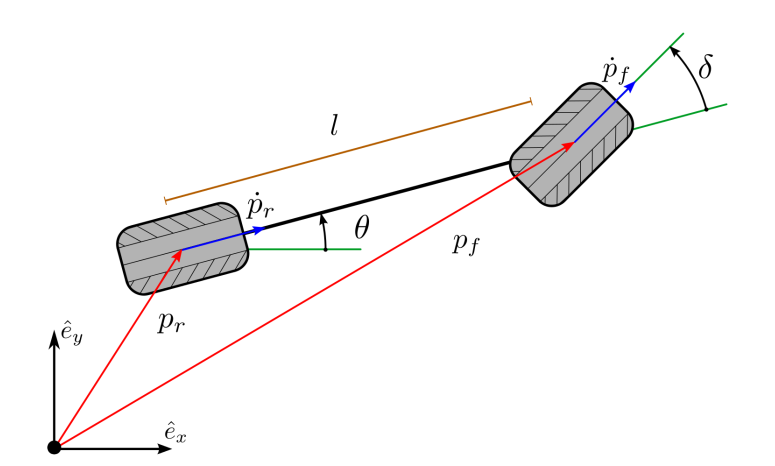
\includegraphics[width=0.5\textwidth]{Figures/Figures_Cap04/single_track_model.png}
    \caption{Modelo cinemático de vía única (\textit{Single-Track Model}).}
    \textit{Nota}. Tomada de \textit{Paden}, 2016 \cite{paden2016survey}.
    \label{fig:single_track_model}
\end{figure}


Por lo general estas expresiones se reordenan en términos del movimiento en cada punto de los vectores base $(\hat{e}_{x}, \hat{e}_{y})$. El movimiento de la llanta trasera a lo largo de $\hat{e}_{x}$ es $x_r := p_r \cdot \hat{e}_x$. Para la dirección $\hat{e}_{y}$, $y_r := p_r \cdot \hat{e}_y$. La velocidad de movimiento es la magnitud de $\dot{p}_r$ con el signo correcto para indicar conducción hacia adelante o en reversa. 

En términos de cantidades escalares $x_r$, $y_r$ y $\theta$, la restricción diferencial es:
\begin{equation}
    \begin{split}
        \dot{x}_r & = v_r \cos{(\theta)} \\
        \dot{y}_r & = v_r \sin{(\theta)} \\
        \dot{\theta}_r & = \frac{v_r}{l}\tan{(\theta)}
    \end{split}
\end{equation}

Alternativamente se puede escribir la misma restricción diferencial en términos del movimiento de la rueda delantera.
\begin{equation}
    \begin{split}
        \dot{x}_f & = v_f \cos{(\theta + \delta)} \\
        \dot{y}_f & = v_f \sin{(\theta + \delta)} \\
        \dot{\theta}_f & = \frac{v_f}{l}\sin{(\delta)}
        \label{eqn:front_whell}
    \end{split}
\end{equation}

pero ahora se utiliza la velocidad de la rueda delantera, esta velocidad está relacionada con la velocidad de la llanta trasera por:
\begin{equation}
    \frac{v_r}{v_f} = \cos{(\delta)}
\end{equation}

Los problemas de control de este modelo pueden implicar el seleccionar un ángulo de dirección $\delta$ dentro de los rangos mecánicos aceptables por el vehículo, $ \delta \in [\delta_{min}, \delta_{max}]$ , y mantener la velocidad de avance en un rango estable, $v_r \in [v_{min}, v_{max}]$. Otro inconveniente importante de este modelo es que permite cambios instantáneos en el ángulo de dirección y por ende provocar cambios bruscos en la dirección.

La continuidad del ángulo de dirección para la rueda delantera se pude imponer añadiendo una velocidad más en la ecuación (\ref{eqn:front_whell}), donde el ángulo de dirección integra una velocidad constante. Entonces, la ecuación (\ref{eqn:front_whell}) se reescribe como:
\begin{equation}
    \begin{split}
        \dot{x}_f & = v_f \cos{(\theta + \delta)} \\
        \dot{y}_f & = v_f \sin{(\theta + \delta)} \\
        \dot{\theta}_f & = \frac{v_f}{l}\sin{(\delta)} \\
        \dot{\delta} & = v_{\delta}
    \end{split}
\end{equation}
Ahora, además de limitar el ángulo de dirección también se puede limitar la velocidad en la dirección para la rueda del frente, $v_{\delta} \in [\dot{\delta}_{min}, \dot{\delta}_{max}]$. Este mismo problema se puede presentar con la velocidad del automóvil descrita por $v_r$ y se puede abordar de la misma manera. El único inconveniente de esta técnica es que el aumento en la dimensión del modelo podría complicar más los problemas de planificación y control del movimiento.

Más adelante se considerará este modelo cinemático para el diseño de las leyes de control que influyan en el movimiento lateral y longitudinal del vehículo autónomo. En concreto, la relación que existe con el movimiento de la rueda delantera y el rango del ángulo de dirección (\textit{steering}).

\section{Leyes de control} \label{sec:leyes_de_control}

Un controlador es un componente que permite procesar información de sensores y generar salidas específicas. La forma en que un controlador opera sobre una señal se conoce como algoritmo de control o ley de control.
% La forma en que un controlador opera sobre una señal de error
El objetivo de una ley de control es ajustar el valor de una señal respecto a un valor conocido, el cual puede provenir de la lectura de un sensor o bien ser el resultado de una operación previa. La diferencia entre valor conocido y valor medido se conoce como error. Una ley de control actúa sobre el error a través de algún mecanismo y manipula el proceso para provocar la salida esperada. Es decir, se pretende que la ley de control pueda compensar efectos de los elementos dinámicos del sistema \cite{gonzalez2015review}.

En este proyecto se busca calcular un error con base en las líneas observadas de los bordes del carril en la sección \ref{sub:ejemplo_para_detección_de_líneas_rectas_con_transformada_Hough} y las líneas reales de los bordes del carril, este error permitirá diseñar un ley de control para el movimiento lateral del vehículo con base en el modelo cinemático. Mediante esta ley de control el vehículo debe ser capaz de controlar el ángulo de dirección (\textit{steering})
en un rango estable para mantenerse dentro del carril en líneas rectas, curvas a la derecha y curvas hacia la izquierda.


\subsection{Diseño e implementación de una ley de control para movimiento lateral del vehículo} \label{sub:diseño_e_implementación_de_una_ley_de_control_para_movimiento_lateral_del_vehículo}

En la búsqueda de mantener el vehículo autónomo alineado y dentro de su carril se deben diseñar leyes de control que faciliten el proceso de seguimiento de carril, el objetivo de las leyes de control es manipular el error entre líneas observadas y líneas reales del carril para posteriormente calcular y establecer valores numéricos para las operaciones tácticas del vehículo, es decir, velocidad para movimiento longitudinal y ángulo de dirección (\textit{steering}) en las llantas delanteras como se vio en el modelo cinemático de la sección \ref{sec:modelo_cinemático_del_vehículo}, esto a fin de generar movimiento lateral.

Como resultado de la detección de carriles en la sección \ref{sub:ejemplo_para_detección_de_líneas_rectas_con_transformada_Hough}, se obtuvieron dos líneas rectas que corresponden a los bordes del carril original en coordenadas cartesianas. Este par de líneas se aprovechan para calcular el ángulo de dirección del vehículo. Con el propósito de mantener el vehículo alineado dentro de el carril es necesario conocer el ángulo con respecto a la horizontal que existe desde el centro del coche hacia cada una de las líneas observadas, este ángulo $\theta$ en cada línea indica si el vehículo se encuentra alineado o desalineado con respecto a las líneas del carril. Bajo este enfoque resulta buena opción trazar una línea desde el centro del vehículo hacia cada borde del carril (izquierdo y derecho) y así conocer la orientación del vehículo en todo momento.

Considerar la imagen \ref{fig:avg_polar_lines}, en ella se muestran dos líneas en color azul desde el centro del vehículo hacia cada uno de los bordes del carril con parámetros distancia y ángulo $(\rho, \theta)$ respectivamente. La imagen permite especificar la geometría de cada una de las líneas. A continuación se describe un algoritmo general para cuantificar los parámetros  $(\rho, \theta)$ de estas líneas imaginarias tomando como referencia la imagen \ref{fig:avg_polar_lines}.

\begin{enumerate}
    \item Formar dos líneas rectas desde el centro del vehículo con coordenadas $C(320, 480)$ hacia los bordes izquierdo y derecho del carril con coordenadas $(x_{pl}, y_{pl})$ y $(x_{pr}, y_{pr})$ respectivamente. Donde, $(x_{px}, y_{px})$ es un punto promedio sobre el borde del carril.
    \item Calcular los parámetros $(\rho, \theta)$ de cada línea con el teorema de Pitágoras:
    \begin{equation}
        \rho = \sqrt{a^2 + b^2}\qquad\qquad\theta = \tan^{-1} \left( \frac{b}{a} \right)
    \end{equation}
    \begin{itemize}
        \item Para la línea del borde izquierdo:
        \begin{equation}
            a_l = 320 - x_{pl}\qquad\qquad b_l = 480 - y_{pl}
        \end{equation}
        \item Para la línea del borde derecho:
        \begin{equation}
            a_r = x_{pr} - 320\qquad\qquad b_r = 480 - y_{pr}
        \end{equation}
    \end{itemize}
    \item Ordenar los parámetros de cada línea en forma polar como:
    \begin{itemize}
        \item Línea izquierda $[\rho_l, \theta_l]$
        \item Línea derecha $[\rho_r, \theta_r]$
    \end{itemize}
\end{enumerate}

\begin{figure}[h]
    \centering
    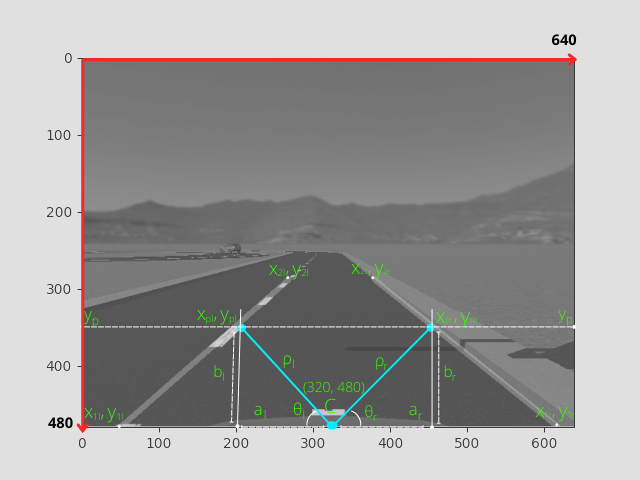
\includegraphics[width=0.75\textwidth]{Figures/Figures_Cap04/avg_polar_lines.png}
    \caption{Geometría de líneas guía del vehículo.}
    \label{fig:avg_polar_lines}
\end{figure}

Una vez que se cuenta con los parámetros de cada una de las rectas desde el centro del vehículo a cada borde del carril es más sencillo calcular las leyes de control. El seguimiento de carril de este trabajo considera cuatro situaciones diferentes en las que podría estar el vehículo.
\begin{enumerate}
    \item Ambas líneas (izquierda y derecha) de los bordes del carril son detectadas indican que el vehículo se encuentra en línea recta.
    \item Solo la línea del borde izquierdo es detectada supone que el vehículo se encuentra en una curva hacía la derecha.
    \item Solo la línea del borde derecho es detectada supone que el vehículo se encuentra en una curva hacía la izquierda.
    \item Ningún borde es detectado indica que el vehículo está fuera de un carril y debe detenerse.
\end{enumerate}

Estas cuatro situaciones son suficientes para que el vehículo pueda determinar la línea con la cual debe guiarse a fin de mantenerse dentro del carril mientras avanza. El seguimiento de carril es logrado usando una ley de control que combina la distancia y el ángulo con respecto al borde del carril. Considerar la figura \ref{fig:línes_desired_lines_detected}, donde las líneas de color verde representan las líneas deseadas si el vehículo se encuentra alineado con los bordes del carril, estas líneas pertenecen a los parámetros $(\rho_{ld}, \theta_{ld})$, $(\rho_{rd}, \theta_{rd})$ para los bordes izquierdo y derecho del carril respectivamente. Líneas en color cyan corresponden a las líneas actualmente observadas de cada borde $(\rho_{l}, \theta_{l})$ y $(\rho_{r}, \theta_{r})$.

\begin{figure}
    \centering
    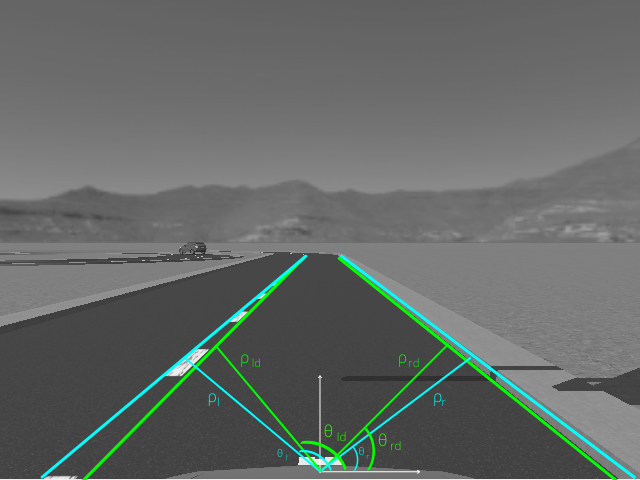
\includegraphics[width=0.75\textwidth]{Figures/Figures_Cap04/lines_control_laws.png}
    \caption{Comparación entre líneas deseadas (verde) y líneas detectadas (cyan).}
    \label{fig:línes_desired_lines_detected}
\end{figure}

La ley de control para movimiento longitudinal del vehículo o velocidad se considera constante en todo momento.
\begin{equation}
    v = C
    \label{eqn:cruise_speed}
\end{equation}

La ley de control en el caso del movimiento lateral o ángulo de dirección es determinado mediante:
\begin{equation}
    \delta = K_\rho e_\rho + K_\theta e_\theta
    \label{eqn:steering_angle}
\end{equation}

Donde $e_\rho$ y $e_\theta$ son errores de distancia y ángulo respectivamente, calculados con las ecuaciones:
\begin{equation}
    e_\rho = \rho_d - \rho_o
    \label{eqn:distance_error}
\end{equation}
\begin{equation}
    e_\theta = \theta_d - \theta_o
    \label{eqn:angle_error}
\end{equation}

Los subíndices $d$ y $o$ en las ecuaciones (\ref{eqn:distance_error})-(\ref{eqn:angle_error}) son etiquetas para ``deseado'' y ``observado'' respectivamente.

Como se mencionó anteriormente dentro del seguimiento del carril se consideran tres casos, las ecuaciones (\ref{eqn:steering_angle})-(\ref{eqn:distance_error})-(\ref{eqn:angle_error}) funcionan bien en los casos donde existen curvas, es decir, cuando solo se detecten bordes del lado izquierdo o bordes del lado derecho. Sin embargo, para seguir el carril en línea recta resulta mejor trabajar con un error promedio de distancia y ángulo en la ecuación (\ref{eqn:steering_angle}) pues ambos bordes del carril se encuentran presentes. Por lo tanto, en este caso las ecuaciones (\ref{eqn:distance_error})-(\ref{eqn:angle_error}) se reescriben de la forma.

\begin{equation}
    e_{\rho_{p}} = \frac{\rho_{l_{d}} - \rho_{l_{o}} + \rho_{r_{d}} - \rho_{r_o}}{2}
    \label{}
\end{equation}
\begin{equation}
    e_{\theta_{p}} = \frac{\theta_{l_{d}} - \theta_{l_{o}} + \theta_{r_{d}} - \theta_{r_{o}}}{2}
    \label{}
\end{equation}

Nuevamente los subíndices $d$ y $o$ son ``deseado'' y ``observado''. Mientras que $p$ es ``promedio'', $r$ y $l$ son \textit{right} y \textit{left} respectivamente.

Entonces la ecuación (\ref{eqn:steering_angle}) queda de la forma:
\begin{equation}
    \delta = K_\rho e_{\rho_{p}} + K_\theta e_{\theta_{p}}
\end{equation}


En cualquiera de los casos anteriores las constantes $K_\rho$ y $K_\theta$ son constantes de sintonización que permiten ajustar el error de distancia y ángulo para precisar el ángulo de dirección que mantendrá el vehículo en cada caso. Estas constantes son obtenidas de manera experimental porque al ser un ambiente simulado no se pueden tener medidas reales de estos parámetros. Una manera fácil de obtener los valores numéricos esperados para $(\rho_{l_{d}}, \theta_{l_{d}})$ y $(\rho_{r_{d}}, \theta_{r_{d}})$ es obtenerlos desde el principio de la simulación con el supuesto de que el vehículo se encuentra bien centrado dentro del carril. Cabe resaltar que se pretenden giros suaves del vehículo para mantener un comportamiento lo más natural y parecido en comparación como lo realizan conductores al frente del volante, bajo estas condiciones el ángulo de dirección disminuye o aumenta en pasos de $1^\circ$.

Con el cálculo de estas ecuaciones, el ángulo de dirección del vehículo siempre se mantiene en un rango seguro para que no salga del carril, mientras que la velocidad es constante en todo momento. Con los cuatro casos anteriores en cuanto a detección de las líneas que conforman el carril se determina que el vehículo puede manejar en situaciones reales guiándose con los bordes del carril. Además, con el objetivo de mantener la integridad del vehículo en líneas curvas se considera una velocidad menor respecto a líneas rectas donde la velocidad es mayor. Sin embargo, en un caso extremo donde el vehículo no sea capaz de detectar un carril por diferentes situaciones la mejor opción es dejar de avanzar, es decir, se considera velocidad $= 0$ y ángulo de dirección $=0$.

Finalmente y con el propósito de demostrar que las operaciones de detección y seguimiento de carril corresponden al resultado esperado se presenta \ref{fig:lane_detect_tracking} como conjunto de imágenes que ilustran cada uno de los escenarios esperados.

\begin{figure}[h]
    \centering
    \begin{subfigure}[b]{0.2\textwidth}
         \centering
         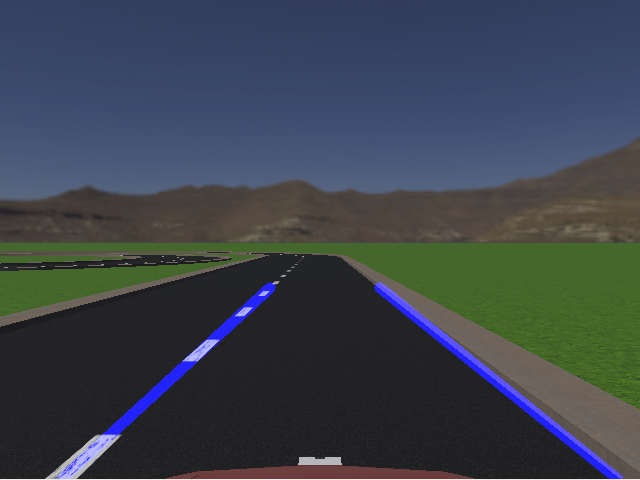
\includegraphics[width=\textwidth]{Figures/Figures_Cap04/both_bordes_detected.png}
         \caption{Ambos bordes}
         \label{fig:both_borders_detected}
    \end{subfigure}
    \hfill
    \begin{subfigure}[b]{0.2\textwidth}
         \centering
         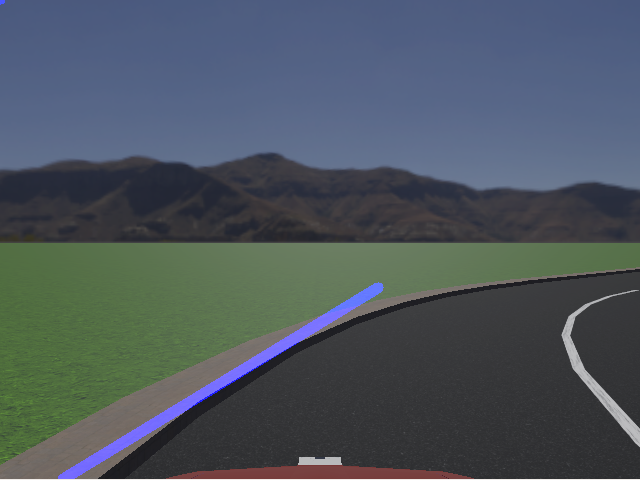
\includegraphics[width=\textwidth]{Figures/Figures_Cap04/left_border_detected.png}
         \caption{Solo borde izquierdo}
         \label{fig:left_border_detected}
     \end{subfigure}
     \hfill
     \begin{subfigure}[b]{0.2\textwidth}
         \centering
         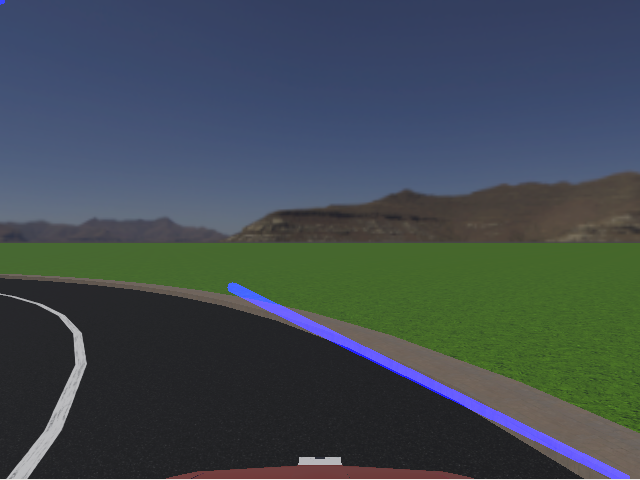
\includegraphics[width=\textwidth]{Figures/Figures_Cap04/right_border_detected.png}
         \caption{Solo borde derecho}
         \label{fig:right_border_detected}
     \end{subfigure}
     \hfill
     \begin{subfigure}[b]{0.2\textwidth}
         \centering
         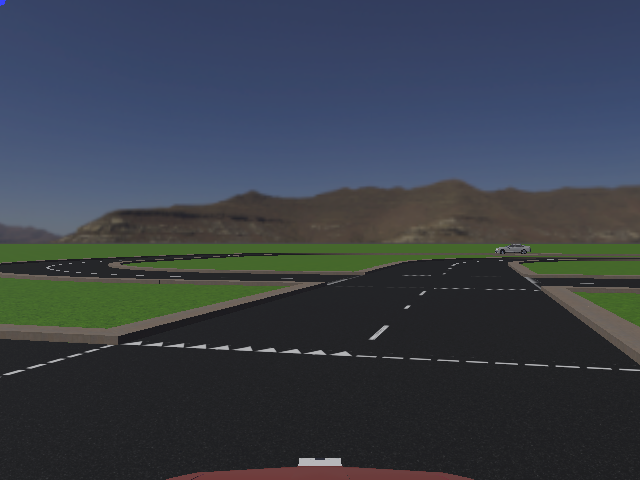
\includegraphics[width=\textwidth]{Figures/Figures_Cap04/no_borders_detected.png}
         \caption{Sin bordes detectados}
         \label{fig:no_edge_detected}
     \end{subfigure}
     
    \caption{Casos considerados según bordes detectados en el seguimiento de carril.}
    \label{fig:lane_detect_tracking}
\end{figure}

En \ref{fig:both_borders_detected} ambos bordes son detectados e indica movimiento en línea recta, las figuras \ref{fig:left_border_detected} y \ref{fig:right_border_detected} corresponden a los casos de curva hacia la derecha y curva hacia la izquierda respectivamente. En curvas a la izquierda debe de prevalecer un ángulo de dirección negativo y en el caso de curvas a la derecha el ángulo tiende a ser positivo. \ref{fig:no_edge_detected} representa una situación donde ningún borde de carril es detectado y la mejor opción es frenar el movimiento. Con este conjunto de imágenes se comprueba el correcto funcionamiento de la detección de carril y seguimiento de carril con las leyes de control diseñadas.
\newpage

%CONCLUSIONES DEL CAPÍTULO
Este capítulo concluye con la implementación de las herramientas matemáticas de detector de bordes de Canny en una imagen y transformada Hough para detección de líneas rectas. Se demostró que se puede desarrollar un sistema de visión artificial que permita el reconocimiento de carriles en la escena a partir de imágenes RGB. Además, se diseñó e implementó un control para establecer operaciones tácticas de movimiento longitudinal y lateral que se ven involucradas en el seguimiento de carril. Con ello, el vehículo fue capaz de recorrer en su totalidad el circuito propuesto en la sección \ref{sec:el_ambiente_de_simulación}, sin obstáculos. 

Sin embargo, en esta sección solo se contemplan situaciones controladas donde no existe ningún otro vehículo a parte del autónomo, lo cual es muy poco probable en el mundo real. De esta manera, el único inconveniente que se puede presentar es que el vehículo deje de detectar carriles para guiar su trayecto. En los siguientes capítulos se aspira a añadir más características al ambiente simulado que sumen en dificultad para la navegación autónoma del vehículo, como es el caso de nuevos vehículos para la detección obstáculos, evasión y seguimiento de vehículos.